\begin{chapter}{Generalizing the wavepacket based algorithm}
\label{ch:multi_family_algorithms}

In this chapter we will extend further the ideas from the last chapter. Most concepts
carry over if we generalize the necessary details as appropriate. Though some pitfalls
appear at the theoretical computations as well as in the implementation.

\section{Inhomogeneous wavepackets}

When we release the restriction of chapter \ref{ch:wave_packet_based_algorithms}
that every wavepacket $\Ket{\Psi}$ can only have a single set of Hagedorn parameters,
all concepts of the last chapter remain valid. But some of the details become more
complicated. In this chapter we'll spot these small differences and present the more
general formulae.

So let's take the first step and drop the homogeneity restriction. For the rest
of this chapter the wavepackets $\Ket{\Psi}$ take the form defined by \eqref{eq:hawp_def_state_vector}
where each component $\Phi_i$ is an expression as defined by \eqref{eq:hawp_def_single}.
And every $\Phi_i$ possesses it's own set of Hagedorn parameters. Hence our wavepackets
are now inhomogeneous ones.

\section{Inner products, integrals and quadrature}

\subsection{An analytical ansatz}

The inner product of two semiclassical wavepackets which have different sets
of Hagedorn parameters denoted by $\{P_k, Q_k, S_k, p_k, q_k\}$ and $\{P_l, Q_l, S_l, p_l, q_l\}$
respectively is written as usual as $\Braket{ \phi^k | \phi^l }$.
This is the expression we want to evaluate now and we can even write down
a closed form solution based on induction and the recursion relation for
Hermite polynomials. The expression for the ground states $\phi_0$ acts as
induction base and is given by

% \begin{multline} \label{eq:multifamily_innerp_ground}
%   \Braket{ \phi_0^k | \phi_0^l } =
%   \sqrt{\frac{2}{B_2 \conj{A_1} + A_2 \conj{B_1}}} \cdot
%     \exp \Biggl(
%       -\frac{A_2 \conj{A_1} \left(\eta_2-\eta_1\right)^2 + B_2 \conj{B_1} \left(a_2-a_1\right)^2}
%             {2 \hbar \left(B_2 \conj{A_1} + A_2 \conj{B_1}\right)}
%     \\
%     -i \frac{\left(a_2-a_1\right)\left(B_2\conj{A_1}\eta_1 + A_2 \conj{B_1}\eta_2\right)}
%               {\hbar \left(B_2 \conj{A_1} + A_2 \conj{B_1}\right)}
%     \Biggr)
% \end{multline}

\begin{multline} \label{eq:multifamily_innerp_ground}
  \Braket{ \phi_0^k | \phi_0^l } =
  \sqrt{\frac{-2 i}{Q_2 \conj{P_1} - P_2 \conj{Q_1}}} \cdot
    \exp \Biggl(
      \frac{i}{2 \varepsilon^2}
      \frac{Q_2 \conj{Q_1} \left(p_2-p_1\right)^2 + P_2 \conj{P_1} \left(q_2-q_1\right)^2}
            {\left(Q_2 \conj{P_1} - P_2 \conj{Q_1}\right)}
    \\
    -\frac{i}{\varepsilon^2}
    \frac{\left(q_2-q_1\right) \left( Q_2 \conj{P_1} p_2 - P_2 \conj{Q_1} p_1\right)}
         {\left(Q_2 \conj{P_1} - P_2 \conj{Q_1}\right)}
    \Biggr) \,.
\end{multline}

For the inner product of higher level functions $\phi_i$ the whole thing gets much
more complicated:

% \begin{multline}
%   \Braket{ \phi_k^k | \phi_l^l } =
%   \frac{1}{\sqrt{l!k!}} 2^{-\frac{l+k}{2}} \Braket{ \phi_0^k | \phi_0^l } \cdot
%   \left(\conj{B_1} A_2 + \conj{A_1} B_2\right)^{-\frac{l+k}{2}} \cdot \\
%   \sum_{j=0}^{\min\left(l,k\right)}
%     \Biggl(
%       \binom{l}{j} \binom{k}{j} j! 4^j \left(\conj{A_2 B_1}-\conj{A_1 B_2}\right)^{\frac{k-j}{2}}
%       \left(A_1 B_2 - A_2 B_1\right)^{\frac{l-j}{2}} \cdot
%       \\
%       H_{k-j}\left(\hbar^{-1/2}\frac{\conj{B_1}\left(a_1-a_2\right)+i \conj{A_1}\left(\eta_1-\eta_2\right)}
%                                     {\sqrt{\conj{A_2 B_1}-\conj{A_1 B_2}}\sqrt{\conj{B_1}A_2+\conj{A_1}B_2}}\right) \cdot
%       \\
%       H_{l-j}\left(-\hbar^{-1/2}\frac{B_2\left(a_1-a_2\right)+i A_2\left(\eta_1-\eta_2\right)}
%                                     {\sqrt{A_1 B_2 - A_2 B_1}\sqrt{\conj{B_1}A_2+\conj{A_1}B_2}}\right)
%     \Biggr)
% \end{multline}

\begin{multline}
  \Braket{ \phi_k^k | \phi_l^l } =
  \frac{1}{\sqrt{l!k!}} 2^{-\frac{l+k}{2}} \Braket{ \phi_0^k | \phi_0^l } \cdot
  \left(i \conj{ P_1} Q_2 - i \conj{Q_1} P_2\right)^{-\frac{l+k}{2}} \cdot \\
  \sum_{j=0}^{\min\left(l,k\right)}
    \Biggl(
      \binom{l}{j} \binom{k}{j} j! 4^j \left(i \conj{Q_2 P_1}-i\conj{Q_1 P_2}\right)^{\frac{k-j}{2}}
      \left(i Q_2  P_1 - i Q_1  P_2\right)^{\frac{l-j}{2}}
      \\
      \cdot H_{k-j}\left(\frac{1}{\varepsilon^2}
                   \frac{\conj{ P_1}\left(q_1-q_2\right)+\conj{Q_1}\left(p_1-p_2\right)}
                        {\sqrt{\conj{Q_2 P_1}-\conj{Q_1 P_2}}\sqrt{\conj{ P_1}Q_2-\conj{Q_1} P_2}}\right)
      \\
      \cdot H_{l-j}\left(-\frac{1}{\varepsilon^2}
                    \frac{-P_2\left(q_1-q_2\right)+Q_2\left(p_1-p_2\right)}
                         {\sqrt{Q_2 P_1 - Q_1 P_2}\sqrt{\conj{P_1}Q_2-\conj{Q_1} P_2}}\right)
    \Biggr) \,.
\end{multline}

For the proofs of these formulae see reference \cite{H_R_quantization_rules}.

Despite we can evaluate the inner product and have a closed form solution for arbitrary
wave functions, these formulae are unsuitable for numerical calculation. There are
several reasons but for example the factorials and binomial coefficients lead to
overflow even for relatively small $k$ and $l$. Further the sum may be numerically
unstable. Thus we need to find a better way to perform these calculations.

\subsection{Quadrature rules for the product of basis functions}

First we notice that each $\phi$ which is given by \eqref{eq:hagedorn_kstate_1d}
is represented through a mathematical expression of the general form

\begin{equation} \label{eq:expression_format}
  C \cdot P_n\ofs{\xi} \cdot \exp \ofs{\theta}
\end{equation}

consisting of an arbitrary constant $C \in \mathbb{C}$, a polynomial $P_n\ofs{\cdot}$
of degree $n$ and an exponential $\exp\ofs{\cdot}$.

We try a new Ansatz for calculating the inner product. Evaluating the braket $\Braket{\phi^k | \phi^l}$
results in a multiplication of two expressions of the form \eqref{eq:expression_format}:

\begin{equation} \label{eq:expression_reformat}
\begin{split}
  \Braket{\phi^k | \phi^l} & =
  \int_\mathbb{R} \conj{C_k P_{n_k}\ofs{\xi_k} \exp \ofs{\theta_k}} C_l P_{n_l}\ofs{\xi_l} \exp \ofs{\theta_l} \,dx \\
  & =   \int_\mathbb{R} \conj{C_k} C_l P_{n_k}\ofs{\conj{\xi_k}} P_{n_l}\ofs{\xi_l} \exp \ofs{\conj{\theta_k}} \exp \ofs{\theta_l} \,dx \,.
\end{split}
\end{equation}

The parts in this expression can be combined by same type. With Gauss Hermite quadrature in
mind we are especially interested in the exponential parts. They have a general form like

\begin{equation} \label{eq:expression_format_exponential}
  \exp\ofs{\theta} = \exp\left(s \cdot \left(x-m\right)^2 + \cdots \right) \,.
\end{equation}

Therefore lets take a closer look at these parts. Our first step consists of combining the exponentials
and distribute the complex conjugate onto the variables affected.

\begin{align} \label{eq:expression_exponentials_combined}
  & \conj{\exp\left(\frac{i}{2\varepsilon^2} P_k Q_k^{-1} \left(x-q_k\right)^2 + \frac{i}{\varepsilon^2} p_k \left( x-q_k \right)\right)}
  \cdot \exp\left(\frac{i}{2\varepsilon^2} P_l Q_l^{-1} \left(x-q_l\right)^2 + \frac{i}{\varepsilon^2} p_l \left( x-q_l \right)\right) \nonumber \\
  = & \exp\left(\conj{\frac{i}{2\varepsilon^2} P_k Q_k^{-1} \left(x-q_k\right)^2 + \frac{i}{\varepsilon^2} p_k \left( x-q_k \right)}
              + \frac{i}{2\varepsilon^2} P_l Q_l^{-1} \left(x-q_l\right)^2 + \frac{i}{\varepsilon^2} p_l \left( x-q_l \right) \right) \nonumber \\
  = & \exp\left( -\frac{i}{2\varepsilon^2} \conj{P_k} \conj{Q_k^{-1}} \left(x-q_k\right)^2 - \frac{i}{\varepsilon^2} p_k \left( x-q_k \right)
              + \frac{i}{2\varepsilon^2} P_l Q_l^{-1} \left(x-q_l\right)^2 + \frac{i}{\varepsilon^2} p_l \left( x-q_l \right) \right) \,.
\end{align}

For the sake of readability we define the following variables

\begin{equation}
\begin{split}
  r_k & \assign P_k Q_k^{-1} \\
  r_l & \assign P_l Q_l^{-1} \,.
\end{split}
\end{equation}

Plugging these into the equation \eqref{eq:expression_exponentials_combined} above
and expanding the squares we get for the exponent

\begin{equation}
  \frac{i}{\varepsilon^2} \left( - \frac{1}{2}\left(\conj{r_k}-r_l\right) x^2
                                 + \left(\conj{r_k}q_k-r_l q_l\right) x
                                 - \frac{1}{2}\left(\conj{r_k}q_k^2 + r_l q_l^2\right)
                                 + \left(p_l-p_k\right) x
                                 + p_k q_k - p_l q_l
                          \right) \,.
\end{equation}

To get back to a form along the lines of \eqref{eq:expression_format_exponential} we
have to complete the square

\begin{equation}
  \frac{i}{\varepsilon^2} \Biggl( \Bigl(x^2 - 2 \underbrace{\frac{\conj{r_k}q_k-r_l q_l}{\conj{r_k}-r_l}}_{q_0} x + q_0^2 - q_0^2\Bigr)
                                 \left(-\frac{\conj{r_k}-r_l}{2}\right)
                                 - \frac{1}{2}\left(\conj{r_k}q_k^2 + r_l q_l^2\right)
                                 + \cdots
                          \Biggr)
\end{equation}

which gives

\begin{equation}
  \frac{i}{\varepsilon^2} \Biggl( \frac{1}{2}\left(r_l-\conj{r_k}\right) \left(x-q_0\right)^2
                                 + \frac{1}{2}\left(\conj{r_k}-r_l\right) q_0^2
                                 - \frac{1}{2}\left(\conj{r_k}q_k^2 + r_l q_l^2\right)
                                 + \cdots
                          \Biggr) \,.
\end{equation}

Finally we got just a new expression which has the general form shown in \eqref{eq:expression_format_exponential}.
In this expression, $q_0$ represents the mean of the Gaussian function while the
prefactor defines the variance or spread. With this results we can now go on and
adapt the Gauss-Hermite quadrature for the case of unequal Hagedorn parameters
and compute the value of an arbitrary integral $\Braket{ \phi^k | \phi^l }$. As
usual we have to transform the quadrature nodes such that they lie in the important
region of space. For this we define the following variables

\begin{equation}
\begin{split}
  r_l & \assign \frac{P_l}{Q_l} \\
  r_k & \assign \frac{P_k}{Q_k} \\
  r_0 & \assign \frac{1}{2} \left(r_l - \conj{r_k}\right) \\
  q_0 & \assign \Re \frac{r_l q_l - \conj{r_k} q_k}{r_l - \conj{r_k}} \\
  Q_0 & \assign \frac{1}{\sqrt{\Im r_0}}
\end{split}
\end{equation}

Now we transform the nodes $\gamma_i$ according to the weighted position mean $q_0$
and the parameter $Q_0$ which changes the spread of the nodes. This yields

\begin{equation}
  \gamma^{\prime}_i \assign q_0 + \varepsilon \cdot \Re Q_0 \cdot \gamma_i
\end{equation}

for the new quadrature nodes which are located in the space around where
the product of $\phi_k$ and $\phi_l$ is maximal. A procedure that calculates
the adapted quadrature results as necessary is given by algorithm \ref{al:mixing_hagedorn_parameters}.

\begin{algorithm}
\caption{Mixing two sets $\Pi_r$ and $\Pi_c$ of Hagedorn parameters}
\label{al:mixing_hagedorn_parameters}
\begin{algorithmic}
  \REQUIRE Two sets $\Pi_r$ and $\Pi_c$ of Hagedorn parameters
  \REQUIRE A quadrature rule $\left(\gamma_i, \omega_i\right)$
  \STATE // Apply the mixing formula to the parameters
  \STATE $r_r \assign \frac{P_r}{Q_r}$
  \STATE $r_c \assign \frac{P_c}{Q_c}$
  \STATE $r_0 \assign \frac{1}{2}\left(r_r - \conj{r_c}\right)$
  \STATE $q_0 \assign \Re \frac{r_r q_r - \conj{r_c} q_c}{r_r - \conj{r_c}}$
  \STATE $Q_0 \assign \frac{1}{\sqrt{\Im r_0}}$
  \STATE // And shift the quadrature nodes
  \STATE $\gamma^\prime \assign q_0 + \varepsilon \Re Q_0 \gamma$
  \RETURN $q_0$ and $Q_0$ and $\gamma^\prime$
\end{algorithmic}
\end{algorithm}

We should get back to the homogeneous case if we choose the sets $\Pi_k$ and
$\Pi_l$ of Hagedorn parameters identical.

\subsection{Integrals of whole components}

Suppose the wave function $\Ket{\Phi_i}$ of a component is given as defined by
\eqref{eq:hawp_def_single}. For an arbitrary but sufficiently smooth real valued
function

\begin{align*}
  f : \mathbb{R} & \rightarrow \mathbb{R} \\
               x & \mapsto f \ofs{x}
\end{align*}

we want to simplify the following expression $\Braket{ \Phi_k | f | \Phi_l }$.
But in contrast to the derivation \eqref{eq:inner_product_single_family} we have
to mind the fact the the different components $\Phi_i$ may belong to two different
parameter families. That is, they have different Hagedorn parameters. Denote by
$\phi^i$ the functions of the form \eqref{eq:hagedorn_kstate_1d} that build the
base of $\Phi_i$ then we can write:

\begin{equation} \label{eq:inner_product_multi_families}
\begin{split}
  \Braket{ \Phi_k | f | \Phi_l } & = \Braket{e^{\frac{iS^k}{\varepsilon^2}} \sum_i c^k_i \phi^k_i |
                                     f | e^{\frac{iS^l}{\varepsilon^2}} \sum_i c^l_i \phi^l_i} \nonumber \\
                                 & = \underbrace{e^{-\frac{i\conj{S^k}}{\varepsilon^2}} e^{\frac{iS^l}{\varepsilon^2}}}_{\neq 1}
                                     \Braket{\sum_i c^k_i \phi^k_i | f | \sum_i c^l_i \phi^l_i} \nonumber \\
                                 & = e^{\frac{i}{\varepsilon^2}\left(S^l-\conj{S^k}\right)}
                                     \sum_{i,j} \conj{c^k_i} c^l_j \Braket{\phi^k_i | f | \phi^l_j} \nonumber \\
                                 & = e^{\frac{i}{\varepsilon^2}\left(S^l-\conj{S^k}\right)}
                                     \sum_{i,j} \conj{c^k_i} c^l_j \int_\mathbb{R} \conj{\phi^k_i\ofs{x}} f\ofs{x} \phi^l_j\ofs{x} dx \,.
\end{split}
\end{equation}

Notice that the phases don't cancel out anymore as each $\Phi_i$ has it's own phase
of different magnitude. We finally reduced the calculation of $\Braket{\Psi | f | \Psi}$ to
a sum of more simple integrals $\Braket{\phi^l_i | f | \phi^k_j}$ over products
of basis functions. This integral can now be evaluated by the means of numerical
quadrature. We can use \ref{al:efficient_quadrature_phi} for this purpose but have
to replace the algorithm that is responsible for calculating $F$.

Integrals of whole wavepackets $\Ket{\Psi}$ can now be split into sums of integrals
over components. That is, we have

\begin{equation}
  \Braket{\Psi | M | \Psi} = \sum_{i,j} \Braket{\Phi_i | M_{i,j} | \Phi_j}
\end{equation}

where $M$ is a $N \times N$ matrix of scalar functions. We will use this identity
for simplifying the calculation of energies.

The figure \ref{fig:quadrature_nodes_mixing} shows the quadrature of an inhomogeneous
wavepacket $\Ket{\Psi}$ that has two components $\Phi_0$ and $\Phi_1$. The Hagedorn
parameters are $\Pi_0 = \left(i,3,0,0.4,3.2\right)$ and $\Pi_0 = \left(i,1.2,0,0.4,2.8\right)$ and
it's coefficients are $c^0 = \left(0,0.3,0.4,0,0,0.6,0.2\right)$ and $c^0 = \left(0,0.8,0.7,0.4\right)$.
We can see the effect of the algorithm \ref{al:mixing_hagedorn_parameters} that
mixes the cyan and the magenta nodes yielding the blue ones which fit best to the
product of the components $\Phi_i$.

\begin{figure}
  \centering
  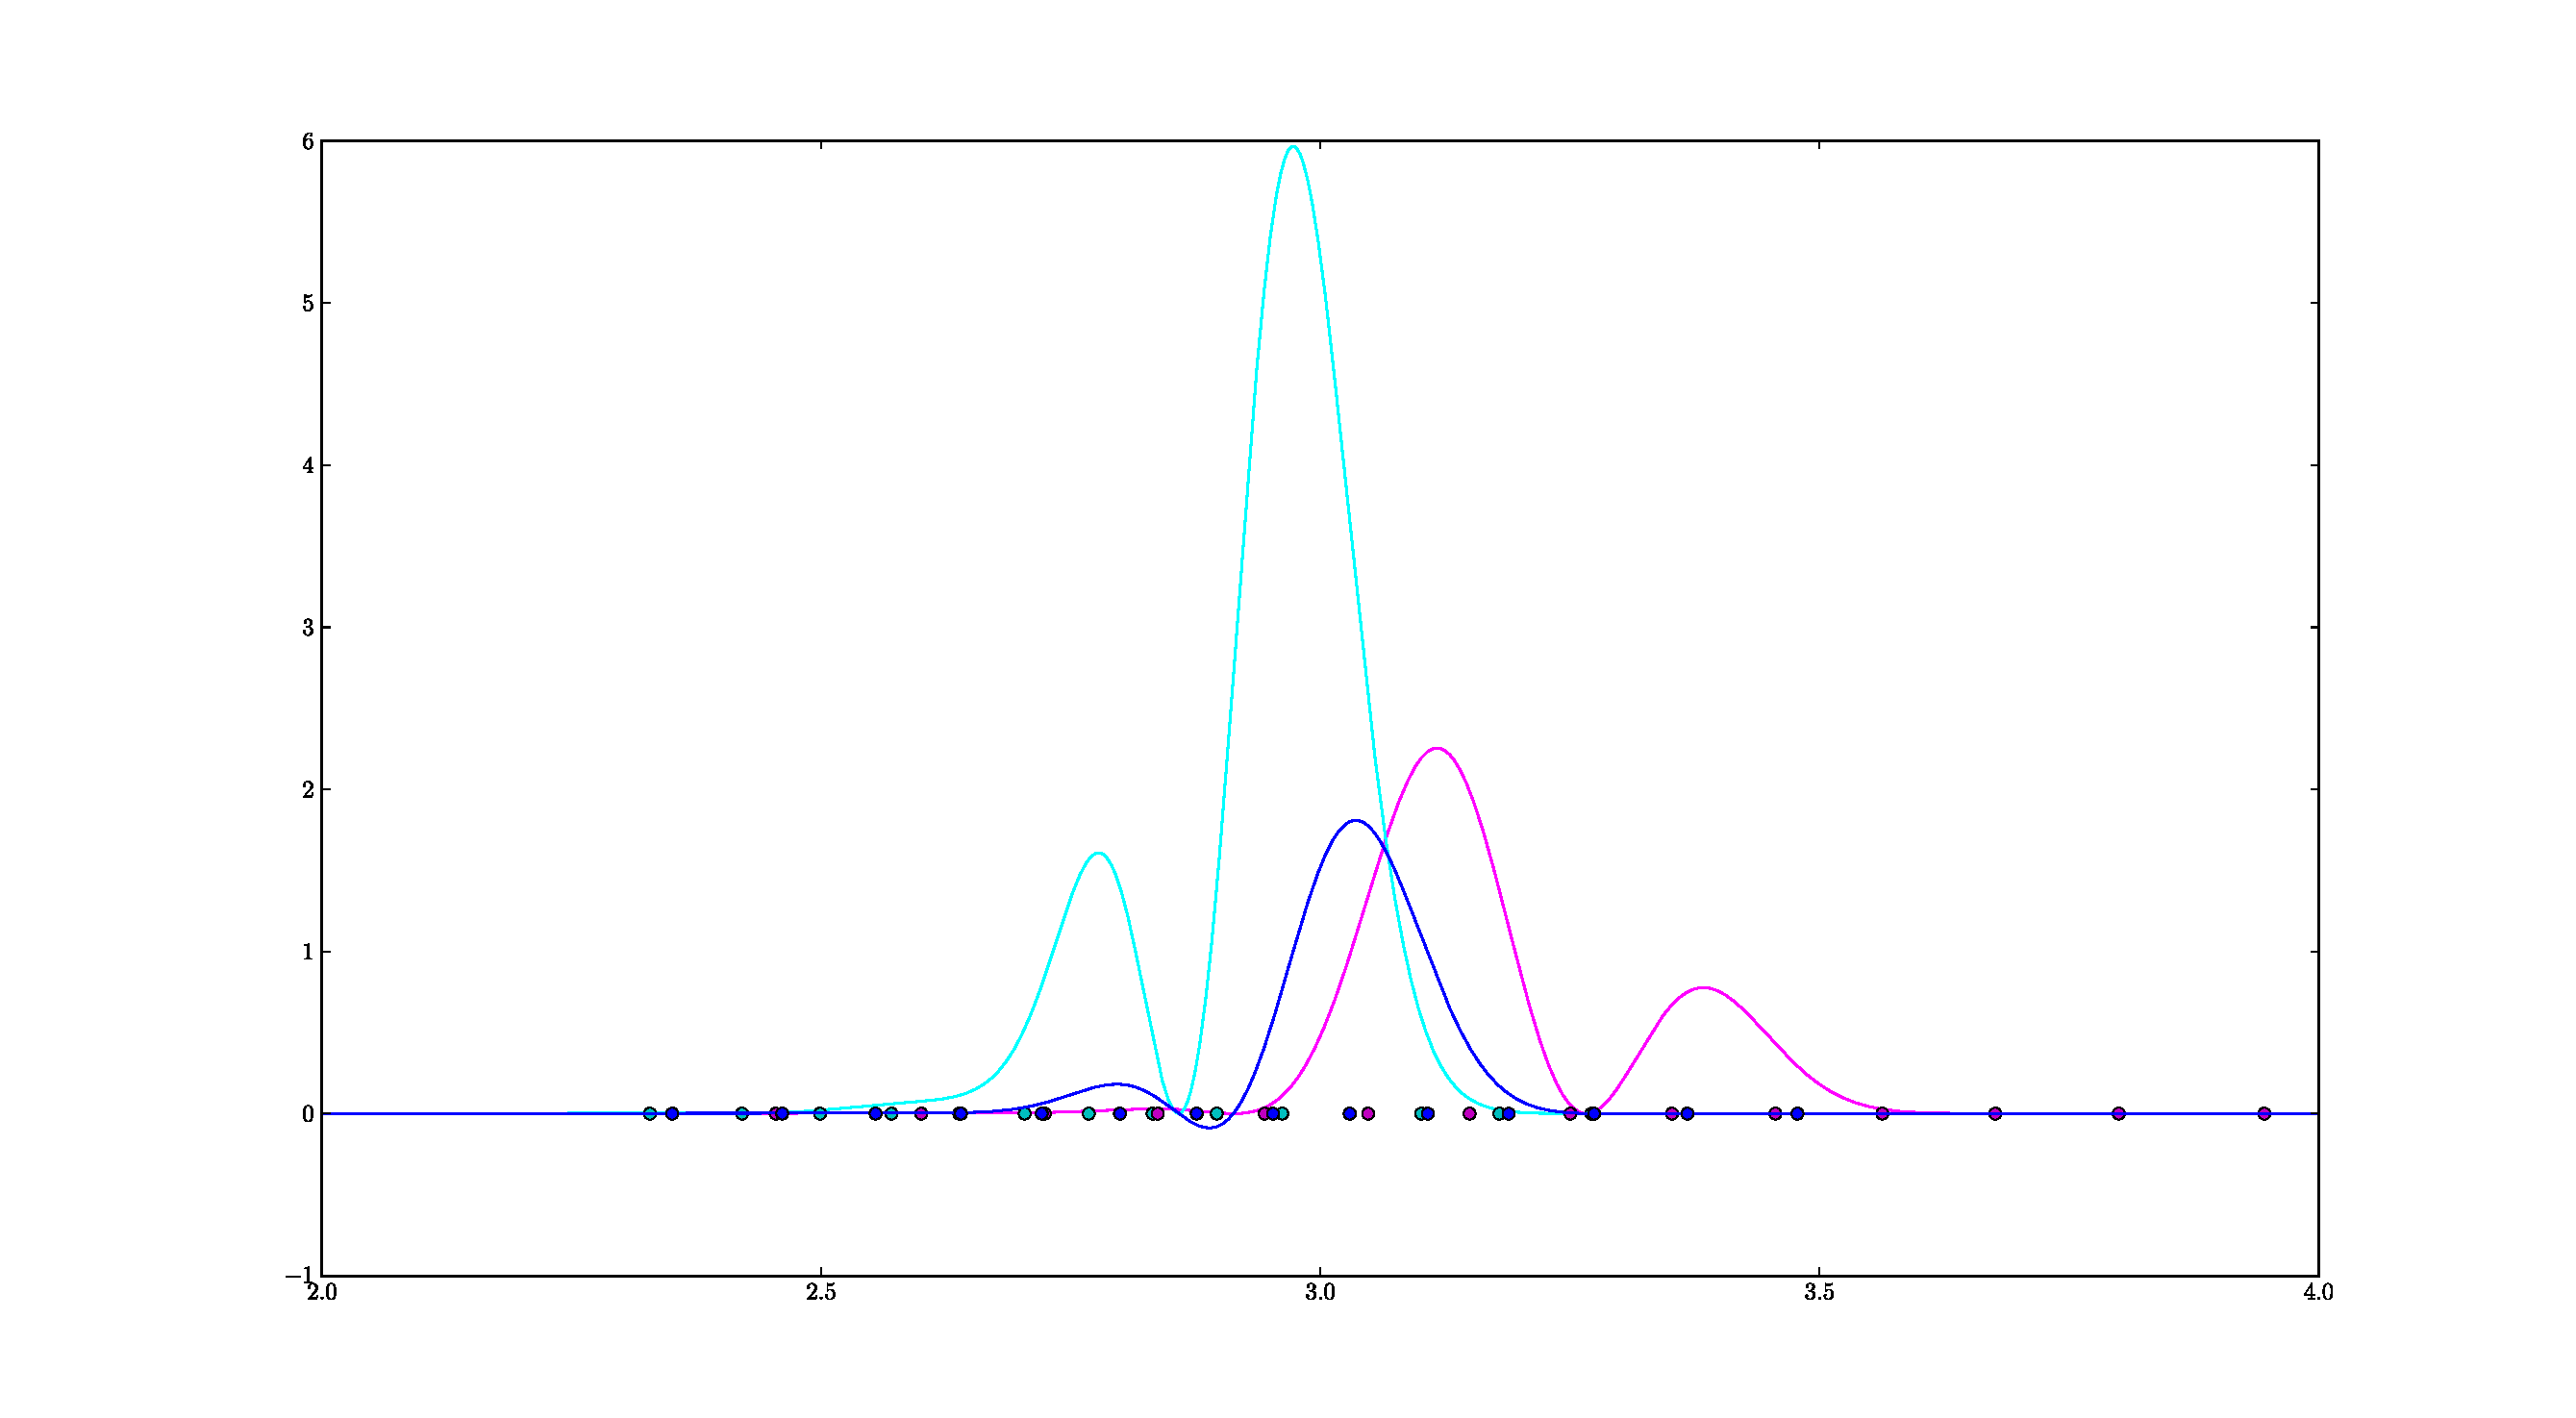
\includegraphics[width=\linewidth]{./figures/quadrature_nodes_mixing.pdf}
  \caption{Example of a quadrature for a given wavepacket $\Psi$. The component
  $\conj{\Phi_0} \Phi_0$ (magenta) and $\conj{\Phi_1} \Phi_1$ (cyan) are shown
  together with their product $\conj{\Phi_0} \Phi_1$ (blue). The quadrature nodes
  have the color of the component defining them.}
  \label{fig:quadrature_nodes_mixing}
\end{figure}


\section{The propagation algorithm for inhomogeneous wavepackets}

In this section we will discuss the same two central points that have to be resolved
for expanding algorithm \ref{al:tp_wave_packets_homog} to inhomogeneous
wavepackets. The most parts are straight forward and obvious but we face some
difficulties too. Let's begin with the easy part, the potential splitting.

\subsection{Splitting of the potential matrix}

For an inhomogeneous vector valued wavepacket $\Ket{\Psi}$ we drop the concept of
a leading index $\chi$. Instead, each energy level $\lambda_i$ is responsible for
propagating the Hagedorn parameters of the packet's component $\Phi_i$. Because of
this reason we have to perform the quadratic Taylor approximation for all $N$
eigenvalues. Let's restrict to one space dimension right now. Then the approximations
read

\begin{equation} \label{eq:pot_taylor_split_inhomog}
\begin{split}
  u_i\ofs{x} & = \lambda_i|_{x=q} + \frac{d}{dx}\lambda_i|_{x=q}\ofs{x-q} + \frac{1}{2} \frac{d^2}{dx^2}\lambda_i|_{x=q} \ofs{x-q}^2 \\
  w_i\ofs{x} & = \lambda_i\ofs{x} - u_i\ofs{x} \quad \forall i \in 0, \ldots, N-1
\end{split}
\end{equation}

where $q$ is the point around which the Taylor expansion is centred.

We can write the potential matrix as a pure quadratic diagonal part $U$ plus a
non-quadratic remainder matrix $W$ once again:

\begin{equation} \label{eq:potiential_splitting_inhomog}
  V =
  \begin{pmatrix}
    u_0 & {}     & 0 \\
    {}  & \ddots & {} \\
    0   & {}     & u_{N-1} \\
  \end{pmatrix}
  +
  \begin{pmatrix}
    v_{0,0} - u_0 & \hdots & v_{0,N-1} \\
    \vdots        & \ddots & \vdots \\
    v_{N-1,0}     & \hdots & v_{N-1,N-1} - u_{N-1} \\
  \end{pmatrix} \,.
\end{equation}

But this time, the matrix $U$ is not just a scaled identity. And we really use all it's entries.
The part $W$ again serves as the matrix for the calculation of $\mathbf{F}$ required in an
adapted version of formula \eqref{eq:splitting_prop_remainder}. We will use $W$
in the algorithm \ref{al:build_block_matrix_inhomog} where we explicitly build
this matrix $\mathbf{F}$.

\subsection{The coefficients}

We stack the coefficient vectors $c^n$ of the $N$ components $\Phi_n$ in the same
way as shown in \eqref{eq:stack_coefficient_vectors_homog}. Thus we need again a
matrix $\mathbf{F}$ analogous to the one shown in \eqref{eq:blocked_F_homog} for the
time evolution of $C$. This time we have to take extra care because of the different
Hagedorn parameters of each $\Phi$. Basically this prevents us from reusing the
evaluated basis functions for all blocks $F_{r,c}$ of $\mathbf{F}$. And we must
not forget the global phase that does not cancel out this time.

\begin{algorithm}
\caption{Build the inhomogeneous block matrix $\mathbf{F} \assign \left(F_{r,c}\right)_{r,c}$}
\label{al:build_block_matrix_inhomog}
\begin{algorithmic}
  \REQUIRE A inhomogeneous wavepacket $\Psi$
  \REQUIRE $W$ a $N \times N$ matrix of scalar functions
  \STATE // Initialize $\mathbf{F}$ as the zero-matrix
  \STATE $\mathbf{F} \in \mathbb{R}^{NK \times NK}, \quad \mathbf{F} \assign \mathbf{0}$
  \STATE // Iterate over all row and column blocks of this matrix
  \FOR{$r = 0$ \TO $N-1$}
    \FOR{$c=0$ \TO $N-1$}
      \STATE // Retrieve the Hagedorn parameters
      \STATE given $\Pi_r$ as $\{P_r,Q_r,S_r,p_r,q_r\}$
      \STATE given $\Pi_c$ as $\{P_c,Q_c,S_c,p_c,q_c\}$
      \STATE Apply the mixing formula to the parameters according to procedure \ref{al:mixing_hagedorn_parameters}
      \STATE // Evaluate the function $W_{r,c}$ for all quadrature nodes $\gamma^\prime$
      \STATE $\left(v_0, \ldots, v_{L-1}\right) \assign W_{r,c}\ofs{\left(\gamma^\prime_0, \ldots, \gamma^\prime_{L-1}\right)}$
      \STATE // Evaluate the basis functions for all quadrature nodes $\gamma^\prime$
      \STATE // Apply algorithm \ref{al:evaluate_basis_functions} for $\Pi_r$ and $\Pi_c$ individually
      \STATE $B_r \assign \left(\beta^r_0, \ldots, \beta^r_{K-1}\right)$
      \STATE $B_c \assign \left(\beta^c_0, \ldots, \beta^c_{K-1}\right)$
      \STATE // Do not forget the non-vanishing phase
      \STATE $\pi_{r,c} \assign \exp\ofs{\frac{i}{\varepsilon^2}\left(S_c - \conj{S_r}\right)}$
      \STATE // Set up a zero matrix
      \STATE $F \in \mathbb{R}^{K \times K}, \quad F \assign \mathbf{0}$
      \STATE // Iterate over all $L$ quadrature pairs $\left(\gamma^\prime_l, \omega_l\right)$
      \FOR{$l=0$ \TO $L-1$}
        \STATE $F \assign F + v_l \varepsilon M_Q \cdot B_r\herm B_c \cdot \omega_l$
      \ENDFOR
      \STATE // Insert the block $F$ into the block matrix $\mathbf{F}$
      \STATE $\mathbf{F}_{r,c} \assign \pi_{r,c} \cdot F$
    \ENDFOR
  \ENDFOR
  \RETURN $\mathbf{F}$
\end{algorithmic}
\end{algorithm}

It becomes immediately clear that this algorithm \ref{al:build_block_matrix_inhomog}
is more expensive than algorithm \ref{al:build_block_matrix_homog}, for example we have to
evaluate the basis for the two components $\Phi_i$ and $\Phi_j$ over and over again
as they differ by their Hagedorn parameters.

\subsection{Pseudo code for the time propagation}

With the preparations of the last section we can now construct an algorithm for the
time propagation of an inhomogeneous wavepacket $\Ket{\Psi}$. This algorithm is
a generalization of the time propagation given in algorithm \ref{al:tp_wave_packets_homog}
to allow for different families of parameters. The core concepts carry over, but
the details are a little bit more complex as we saw in the last sections.

\begin{algorithm}
\caption{Time propagation of a inhomogeneous wavepacket $\Ket{\Psi}$}
\label{al:tp_wave_packets_inhomog}
\begin{algorithmic}
  \REQUIRE A semiclassical wavepacket $\Ket{\Psi\ofs{t}}$
  \REQUIRE The sets $\Pi_0, \ldots \Pi_{N-1}$ of Hagedorn parameters of $\Psi$
  \STATE // Propagate with the kinetic operator
  \FOR{$n \assign 0$ \TO $N-1$}
    \STATE $q_n^{\left(j+\frac{1}{2}\right)} \assign q_n^{\left(j\right)} + \frac{\tau}{2} p_n^{\left(j\right)}$
    \STATE $Q_n^{\left(j+\frac{1}{2}\right)} \assign Q_n^{\left(j\right)} + \frac{\tau}{2} P_n^{\left(j\right)}$
    \STATE $S_n^{\left(j+\frac{1}{2},-\right)} \assign S_n^{\left(j\right)} + \frac{\tau}{4} p_n^{\left(j\right)}\T p_n^{\left(j\right)}$
  \ENDFOR
  \STATE // Propagate with the local quadratic potential
  \FOR{$n \assign 0$ \TO $N-1$}
    \STATE $p_n^{\left(j+1\right)} \assign p_n^{\left(j\right)} - \tau \, \nabla \lambda_n\ofs{q_n^{\left(j+1/2\right)}}$
    \STATE $P_n^{\left(j+1\right)} \assign P_n^{\left(j\right)} - \tau \, \nabla^2 \lambda_n\ofs{q_n^{\left(j+1/2\right)}} Q_n^{\left(j+1/2\right)}$
    \STATE $S_n^{\left(j+1/2,+\right)} \assign S_n^{\left(j+1/2,-\right)} - \tau \, \lambda_n\ofs{q_n^{\left(j+1/2\right)}}$
  \ENDFOR
  \STATE // Propagate with the non-quadratic remainder
  \STATE // Stack the coefficient vectors $c^n$ of all components
  \STATE $C^{\left(j\right)} \assign \left(c^0, \hdots, c^{N-1}\right)\T$

  \STATE // Assemble the matrix $\mathbf{F}$ using algorithm \ref{al:build_block_matrix_inhomog}
  \STATE $\mathbf{F}^{\left(j+1/2\right)} \assign \left(F_{r,c}\right)_{r,c} \quad \forall r,c \in 0,\ldots,N-1$
  \STATE // Propagate the coefficients
  \STATE $C^{\left(j+1\right)} \assign \exp\ofs{-\tau \frac{i}{\varepsilon^2} \mathbf{F}^{\left(j+1/2\right)}} C^{\left(j\right)}$
  \STATE // Split the coefficients
  \STATE $\left(c^0, \ldots, c^{N-1}\right) \assign C^{\left(j+1\right)}$

  \STATE // Propagate with the kinetic operator again
  \FOR{$n \assign 0$ \TO $N-1$}
    \STATE $q_n^{\left(j+1\right)} \assign q_n^{\left(j+1/2\right)} + \frac{\tau}{2} p_n^{\left(j+1\right)}$
    \STATE $Q_n^{\left(j+1\right)} \assign Q_n^{\left(j+1/2\right)} + \frac{\tau}{2} P_n^{\left(j+1\right)}$
    \STATE $S_n^{\left(j+1\right)} \assign S_n^{\left(j+1/2,+\right)} + \frac{\tau}{4} p_n^{\left(j+1\right)}\T p_n^{\left(j+1\right)}$
  \ENDFOR
  \RETURN $\Ket{\Psi\ofs{t+\tau}}$
\end{algorithmic}
\end{algorithm}

\section{Basis transformation}
\label{sec:basis_transformation_hagedorn_inhomog}

Basis transformations from and to the eigenbasis work in principle exactly like
defined in section \ref{sec:basis_transformation_hagedorn}. We can again write
this as a matrix multiplication with a big block matrix $\mathbf{F}$:

\begin{equation*}
  \left(\begin{array}{c}
    d^0 \\
    \hline
    \vdots \\
    \hline
    d^{N-1}
  \end{array}\right)
  =
  \left(
  \begin{array}{c|c|c}
    \Braket{\varphi_0|m_{0,0}|\varphi_0} & \hdots & \Braket{\varphi_0|m_{0,N-1}|\varphi_{N-1}} \\
    \hline
    \vdots & {} & \vdots \\
    \hline
    \Braket{\varphi_{N-1}|m_{N-1,0}|\varphi_0} & \hdots & \Braket{\varphi_{N-1}|m_{N-1,N-1}|\varphi_{N-1}} \\
  \end{array}\right)
  \left(\begin{array}{c}
    c^0 \\
    \hline
    \vdots \\
    \hline
    c^{N-1}
  \end{array}\right)
\end{equation*}

where each $\varphi_n$ collects the basis functions $\phi_k$ of component $\Phi_n$
in a vector and $d^i$ denotes the transformed coefficient vectors. This time all $\varphi_n$ differ because we deal with inhomogeneous
wavepackets. Only for the calculation of the submatrices we now switch to algorithm
\ref{al:build_block_matrix_inhomog} instead of \ref{al:build_block_matrix_homog}
in the homogeneous case.

\section{Observables}

The calculation of observables is roughly the same as with homogeneous wavepackets
but we encounter some details which are not present in the less general version.
However, we will only outline the changes with respect to the corresponding
section in chapter \ref{ch:wave_packet_based_algorithms}.

\subsection{Norm calculation}

The calculation of the norm of our wavepackets is as simple as in the homogeneous
case. We only need the inner products for all components. And the nice thing is
that all the integrals consist of only bras and kets with an equal family of parameters

\begin{equation}
  \norm{\Psi}^2  = \Braket{\Psi|\Psi} = \sum_i^{N-1} \Braket{\Phi_i | \Phi_i} = \sum_i^{N-1} \norm{c^i}^2 \,.
\end{equation}

The only tricky part here may be the transformation to the eigenbasis to get the
norms of all components we are interested in. But this change of basis can be
done easily as shown in \ref{sec:basis_transformation_hagedorn_inhomog}.

\subsection{Potential and kinetic energy}

We are interested in the energies of the wavepacket and its components in the
eigenbasis. Hence we need the generalized basis transformation defined above here too. Besides
this, everything remains valid and especially the formulae \eqref{eq:potential_energy_eigen_homog}
and \eqref{eq:kinetic_energy_eigen_homog} for the potential and the kinetic energy still hold.

\end{chapter}